\begin{frame}
    \frametitle{ACID vs. BASE}

    \begin{columns}
        \column{.5\textwidth}

        \begin{block}{ACID}
            \begin{itemize}
                \item \textit{\red{A}tomicity}
                \item \textit{\red{C}onsistency}
                \item \textit{\red{I}solation}
                \item \textit{\red{D}urability}
            \end{itemize}
        \end{block}

        \column{.5\textwidth}

        \begin{block}{BASE}
            \begin{itemize}
                \item \textit{\red{Ba}sically Available}
                \item \textit{\red{S}oft state}
                \item \textit{\red{E}ventual consistency}
            \end{itemize}
        \end{block}
    \end{columns}

\end{frame}

\begin{frame}
    \frametitle{ACID vs. BASE}

    \centering
    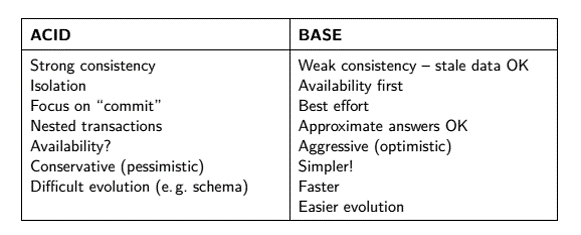
\includegraphics[width=\textwidth]{acid-vs-base.jpg}
\end{frame}